
\documentclass[11pt]{article}
\usepackage[a4paper,margin=1in]{geometry}
\usepackage{amsmath,amssymb}
\usepackage{graphicx}
\usepackage[dvipsnames]{xcolor}
\usepackage{hyperref}
\usepackage{enumitem}
\usepackage{tabularx}
\usepackage{longtable}
\usepackage{booktabs}
\usepackage[most]{tcolorbox}
\usepackage{titlesec}
\usepackage{xurl}
\usepackage{fancyhdr}
\usepackage{setspace}
\usepackage{tikz}
\usetikzlibrary{positioning,arrows.meta}
\usepackage[T1]{fontenc}
\usepackage{lmodern}
\setlength{\parindent}{0pt}
\setlength{\parskip}{8pt}
\setlength{\headheight}{14pt}
\setstretch{1.12}
\setlist[itemize]{leftmargin=1.5em, nosep}
\setlist[enumerate]{leftmargin=1.5em, nosep}
\providecommand{\tightlist}{\setlength{\itemsep}{0pt}\setlength{\parskip}{0pt}}
\hypersetup{colorlinks=true,linkcolor=MidnightBlue,urlcolor=MidnightBlue}
\pagestyle{fancy}
\fancyhf{}
\rhead{\thepage}
\renewcommand{\headrulewidth}{0pt}
\renewcommand{\footrulewidth}{0pt}
\titleformat{\section}{\Large\bfseries\color{MidnightBlue}}{\thesection}{0.6em}{}
\titleformat{\subsection}{\bfseries}{}{0em}{}


\begin{document}

\begin{center}\LARGE\bfseries Probabilistic Reasoning over Time\end{center}

\begin{center}\large Block 4 Day 3\end{center}

\begin{tcolorbox}[colback=MidnightBlue!4,colframe=MidnightBlue,title={Session Overview},fonttitle=\bfseries,breakable]
\textbf{Session objective:} Build temporal reasoning confidence across filtering, prediction, smoothing, and model choice, while introducing the full form of dynamic Bayesian networks clearly.

\textbf{Timing target (min):} 71

\textbf{Topic anchors:} hidden markov model; kalman filter; dynamic bayesian network; filtering; smoothing; prediction

\textbf{Padlet board:} \url{https://padlet.com/qmul/b4-d3-fd8ow6q41h6uka56}
\end{tcolorbox}

\section*{Exercises}

\begin{tcolorbox}[colback=white,colframe=MidnightBlue,title={Q1 Core Concept Check},fonttitle=\bfseries,breakable]
\begin{center}
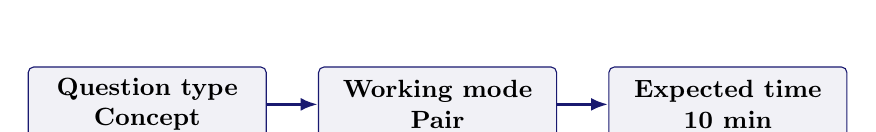
\begin{tikzpicture}[
node distance=0.65cm,
box/.style={draw=MidnightBlue, rounded corners=2pt, minimum height=0.95cm, align=center, font=\small\bfseries, fill=MidnightBlue!6, text width=0.23\linewidth},
arrow/.style={-{Latex[length=2.2mm]}, very thick, MidnightBlue}
]
\node[box] (type) {Question type\\Concept};
\node[box, right=of type] (mode) {Working mode\\Pair};
\node[box, right=of mode] (time) {Expected time\\10 min};
\draw[arrow] (type) -- (mode);
\draw[arrow] (mode) -- (time);
\end{tikzpicture}
\end{center}

{\large\bfseries\color{MidnightBlue} Prompt}\par\medskip
Define filtering, prediction, smoothing, and most-likely sequence in simple language. Give one small scenario example for each, and make the time reference clear in each answer.

{\large\bfseries\color{MidnightBlue} Task details}\par\medskip
\begin{itemize}\item \textbf{Type:} concept
\item \textbf{Mode:} pair
\item \textbf{Time:} 10 min
\item \textbf{Deliverable:} definitions with examples
\item \textbf{Assessment focus:} distinguish the four core temporal questions clearly
\item \textbf{Expected length:} 4 definitions + 4 examples\end{itemize}

{\large\bfseries\color{MidnightBlue} How to submit}\par\medskip
Post one pair Padlet comment with four short definitions and four matching examples.

{\large\bfseries\color{MidnightBlue} Discussion in class}\par\medskip
Which temporal question is easiest to confuse with another one?

{\large\bfseries\color{MidnightBlue} Why this helps}\par\medskip
Useful for short theory questions that separate the main temporal inference tasks.

{\large\bfseries\color{MidnightBlue} References}\par\medskip
\begin{itemize}\item Russell \& Norvig (2021) AIMA 4e, Ch.14, pp.461-499
\item Poole \& Mackworth (2023) 3e, Ch.9, pp.375-458\end{itemize}
\end{tcolorbox}

\begin{tcolorbox}[colback=white,colframe=MidnightBlue,title={Q2 Structured Problem},fonttitle=\bfseries,breakable]
\begin{center}
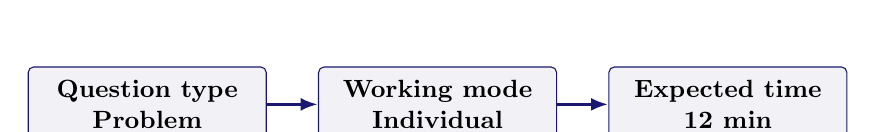
\begin{tikzpicture}[
node distance=0.65cm,
box/.style={draw=MidnightBlue, rounded corners=2pt, minimum height=0.95cm, align=center, font=\small\bfseries, fill=MidnightBlue!6, text width=0.23\linewidth},
arrow/.style={-{Latex[length=2.2mm]}, very thick, MidnightBlue}
]
\node[box] (type) {Question type\\Problem};
\node[box, right=of type] (mode) {Working mode\\Individual};
\node[box, right=of mode] (time) {Expected time\\12 min};
\draw[arrow] (type) -- (mode);
\draw[arrow] (mode) -- (time);
\end{tikzpicture}
\end{center}

{\large\bfseries\color{MidnightBlue} Prompt}\par\medskip
In a warehouse-monitoring example, let the hidden state be Busy or NotBusy. Suppose P(Busy\_t)=0.55, P(Busy\_t+1\textbar Busy\_t)=0.75, P(Busy\_t+1\textbar NotBusy\_t)=0.25, P(Alert\textbar Busy)=0.80, and P(Alert\textbar NotBusy)=0.30. After observing Alert=true at time t+1, compute the filtered belief P(Busy\_t+1 \textbar{} Alert\_t+1=true).

{\large\bfseries\color{MidnightBlue} Task details}\par\medskip
\begin{itemize}\item \textbf{Type:} problem
\item \textbf{Mode:} individual
\item \textbf{Time:} 12 min
\item \textbf{Deliverable:} filtering update
\item \textbf{Assessment focus:} execute one forward update using transition and sensor models
\item \textbf{Expected length:} 5 calculation lines\end{itemize}

{\large\bfseries\color{MidnightBlue} How to submit}\par\medskip
Post your own Padlet comment showing the prediction step, the evidence update, the normalization step, and the final belief.

{\large\bfseries\color{MidnightBlue} Discussion in class}\par\medskip
Why do we need both the transition model and the observation model here?

{\large\bfseries\color{MidnightBlue} Why this helps}\par\medskip
Direct practice for one-step temporal belief updates using a scenario different from the exam examples.

{\large\bfseries\color{MidnightBlue} References}\par\medskip
\begin{itemize}\item Russell \& Norvig (2021) AIMA 4e, Ch.14, pp.461-499
\item Poole \& Mackworth (2023) 3e, Ch.9, pp.375-458\end{itemize}
\end{tcolorbox}

\begin{tcolorbox}[colback=white,colframe=MidnightBlue,title={Q3 Structured Problem},fonttitle=\bfseries,breakable]
\begin{center}
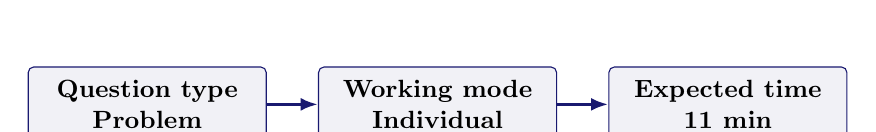
\begin{tikzpicture}[
node distance=0.65cm,
box/.style={draw=MidnightBlue, rounded corners=2pt, minimum height=0.95cm, align=center, font=\small\bfseries, fill=MidnightBlue!6, text width=0.23\linewidth},
arrow/.style={-{Latex[length=2.2mm]}, very thick, MidnightBlue}
]
\node[box] (type) {Question type\\Problem};
\node[box, right=of type] (mode) {Working mode\\Individual};
\node[box, right=of mode] (time) {Expected time\\11 min};
\draw[arrow] (type) -- (mode);
\draw[arrow] (mode) -- (time);
\end{tikzpicture}
\end{center}

{\large\bfseries\color{MidnightBlue} Prompt}\par\medskip
Match each scenario to the best model and explain why: (1) a robot with continuous position and velocity, (2) a weather model with a single hidden discrete state, and (3) a campus-assistant model tracking several linked hidden variables over time. Choose from hidden Markov model (HMM), Kalman filter, and dynamic Bayesian network (DBN).

{\large\bfseries\color{MidnightBlue} Task details}\par\medskip
\begin{itemize}\item \textbf{Type:} problem
\item \textbf{Mode:} individual
\item \textbf{Time:} 11 min
\item \textbf{Deliverable:} model-choice note
\item \textbf{Assessment focus:} distinguish hidden Markov models, Kalman filters, and dynamic Bayesian networks
\item \textbf{Expected length:} 3 labelled choices\end{itemize}

{\large\bfseries\color{MidnightBlue} How to submit}\par\medskip
Post your own Padlet comment with three labelled choices and one reason each.

{\large\bfseries\color{MidnightBlue} Discussion in class}\par\medskip
Which scenario most clearly requires a dynamic Bayesian network rather than a simpler hidden Markov model?

{\large\bfseries\color{MidnightBlue} Why this helps}\par\medskip
Useful for model-selection questions that test assumptions instead of arithmetic.

{\large\bfseries\color{MidnightBlue} References}\par\medskip
\begin{itemize}\item Russell \& Norvig (2021) AIMA 4e, Ch.14, pp.461-499
\item Poole \& Mackworth (2023) 3e, Ch.9, pp.375-458\end{itemize}
\end{tcolorbox}

\begin{tcolorbox}[colback=white,colframe=MidnightBlue,title={Q4 Collaborative Mini-Case},fonttitle=\bfseries,breakable]
\begin{center}
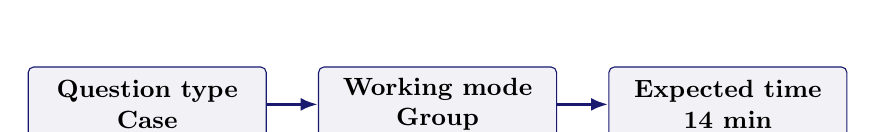
\begin{tikzpicture}[
node distance=0.65cm,
box/.style={draw=MidnightBlue, rounded corners=2pt, minimum height=0.95cm, align=center, font=\small\bfseries, fill=MidnightBlue!6, text width=0.23\linewidth},
arrow/.style={-{Latex[length=2.2mm]}, very thick, MidnightBlue}
]
\node[box] (type) {Question type\\Case};
\node[box, right=of type] (mode) {Working mode\\Group};
\node[box, right=of mode] (time) {Expected time\\14 min};
\draw[arrow] (type) -- (mode);
\draw[arrow] (mode) -- (time);
\end{tikzpicture}
\end{center}

{\large\bfseries\color{MidnightBlue} Prompt}\par\medskip
Design a temporal reasoning pipeline for smart transportation incident response. Include evidence sources, update cadence, one uncertainty threshold, and what the system should do when confidence becomes too low.

{\large\bfseries\color{MidnightBlue} Task details}\par\medskip
\begin{itemize}\item \textbf{Type:} case
\item \textbf{Mode:} group
\item \textbf{Time:} 14 min
\item \textbf{Deliverable:} pipeline sketch
\item \textbf{Assessment focus:} design a temporal reasoning pipeline with update cadence and uncertainty thresholds
\item \textbf{Expected length:} 5 steps\end{itemize}

{\large\bfseries\color{MidnightBlue} How to submit}\par\medskip
Post one group Padlet comment with the pipeline stages, the timing choice, and one fallback action.

{\large\bfseries\color{MidnightBlue} Discussion in class}\par\medskip
How often should the system update before compute cost becomes a problem?

{\large\bfseries\color{MidnightBlue} Why this helps}\par\medskip
Supports design questions on temporal reasoning systems without matching the exam wording directly.

{\large\bfseries\color{MidnightBlue} References}\par\medskip
\begin{itemize}\item Russell \& Norvig (2021) AIMA 4e, Ch.14, pp.461-499
\item Poole \& Mackworth (2023) 3e, Ch.9, pp.375-458\end{itemize}
\end{tcolorbox}

\begin{tcolorbox}[colback=white,colframe=MidnightBlue,title={Q5 Exam-Style Constructed Response},fonttitle=\bfseries,breakable]
\begin{center}
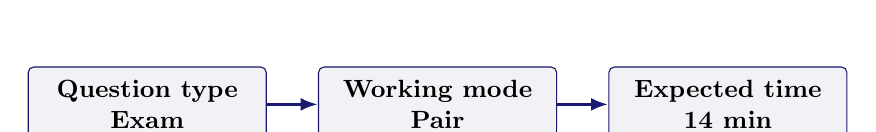
\begin{tikzpicture}[
node distance=0.65cm,
box/.style={draw=MidnightBlue, rounded corners=2pt, minimum height=0.95cm, align=center, font=\small\bfseries, fill=MidnightBlue!6, text width=0.23\linewidth},
arrow/.style={-{Latex[length=2.2mm]}, very thick, MidnightBlue}
]
\node[box] (type) {Question type\\Exam};
\node[box, right=of type] (mode) {Working mode\\Pair};
\node[box, right=of mode] (time) {Expected time\\14 min};
\draw[arrow] (type) -- (mode);
\draw[arrow] (mode) -- (time);
\end{tikzpicture}
\end{center}

{\large\bfseries\color{MidnightBlue} Prompt}\par\medskip
Explain why a dynamic Bayesian network can represent some temporal problems better than a simple hidden Markov model. Your answer should mention structure, number of variables, and why the richer model can still be harder to use.

{\large\bfseries\color{MidnightBlue} Task details}\par\medskip
\begin{itemize}\item \textbf{Type:} exam
\item \textbf{Mode:} pair
\item \textbf{Time:} 14 min
\item \textbf{Deliverable:} structured explanation
\item \textbf{Assessment focus:} explain why dynamic Bayesian networks are richer than simple HMMs
\item \textbf{Expected length:} 180-230 words\end{itemize}

{\large\bfseries\color{MidnightBlue} How to submit}\par\medskip
Post one pair Padlet comment with a clear claim, two technical reasons, and one trade-off.

{\large\bfseries\color{MidnightBlue} Discussion in class}\par\medskip
When is the extra modelling power of a dynamic Bayesian network not worth the extra complexity?

{\large\bfseries\color{MidnightBlue} Why this helps}\par\medskip
Matches exam-style explanation about temporal model choice while avoiding a copy of likely paper wording.

{\large\bfseries\color{MidnightBlue} References}\par\medskip
\begin{itemize}\item Russell \& Norvig (2021) AIMA 4e, Ch.14, pp.461-499
\item Poole \& Mackworth (2023) 3e, Ch.9, pp.375-458\end{itemize}
\end{tcolorbox}

\begin{tcolorbox}[colback=white,colframe=MidnightBlue,title={Q6 Stretch Extension},fonttitle=\bfseries,breakable]
\begin{center}
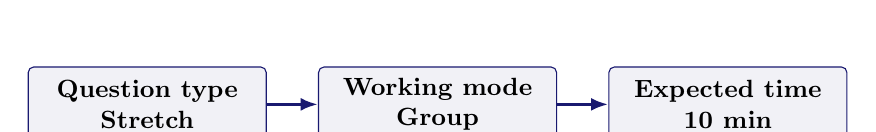
\begin{tikzpicture}[
node distance=0.65cm,
box/.style={draw=MidnightBlue, rounded corners=2pt, minimum height=0.95cm, align=center, font=\small\bfseries, fill=MidnightBlue!6, text width=0.23\linewidth},
arrow/.style={-{Latex[length=2.2mm]}, very thick, MidnightBlue}
]
\node[box] (type) {Question type\\Stretch};
\node[box, right=of type] (mode) {Working mode\\Group};
\node[box, right=of mode] (time) {Expected time\\10 min};
\draw[arrow] (type) -- (mode);
\draw[arrow] (mode) -- (time);
\end{tikzpicture}
\end{center}

{\large\bfseries\color{MidnightBlue} Prompt}\par\medskip
Propose a drift-monitoring plan for an energy-grid temporal model in production. Include at least one signal about model inputs, one about model outputs, and one trigger for human review.

{\large\bfseries\color{MidnightBlue} Task details}\par\medskip
\begin{itemize}\item \textbf{Type:} stretch
\item \textbf{Mode:} group
\item \textbf{Time:} 10 min
\item \textbf{Deliverable:} drift-monitoring plan
\item \textbf{Assessment focus:} detect drift and failure in a deployed temporal model
\item \textbf{Expected length:} 4-5 checks\end{itemize}

{\large\bfseries\color{MidnightBlue} How to submit}\par\medskip
Post one group Padlet comment with four or five checks and one escalation trigger.

{\large\bfseries\color{MidnightBlue} Discussion in class}\par\medskip
Which drift signal would you watch first in a safety-critical temporal system?

{\large\bfseries\color{MidnightBlue} Why this helps}\par\medskip
Good extension for questions that connect temporal inference to monitoring and trust.

{\large\bfseries\color{MidnightBlue} References}\par\medskip
\begin{itemize}\item Russell \& Norvig (2021) AIMA 4e, Ch.14, pp.461-499
\item Poole \& Mackworth (2023) 3e, Ch.9, pp.375-458\end{itemize}
\end{tcolorbox}

\section*{Submission Instructions}

Use the seeded Padlet posts for Q1--Q6. Q2 and Q3 are individual. Q1 and Q5 are pair tasks. Q4 and Q6 should be one joint group comment. Start each comment with your names or group label.

\section*{Whole-Class Debrief Prompts}

\begin{itemize}
\tightlist
\item
  Which temporal question needs the strongest intuition to answer correctly?
\item
  Why was the filtering calculation easier or harder than yesterday's BN calculations?
\item
  When does a temporal model need a human fallback instead of one more automatic update?
\end{itemize}

\section*{Exam Transfer Note (Day-Level)}

Maps to exam questions on filtering, prediction, smoothing, most-likely sequence, and choosing HMM, Kalman filter, or dynamic Bayesian network for real domains.

\end{document}
